\documentclass[aspectratio=169, professionalfonts, 10pt]{beamer}
\usepackage[utf8]{inputenc}
\usepackage[T1]{fontenc}
\usepackage{graphicx}
\usepackage{booktabs}
\usepackage{amsmath}
\usepackage{amssymb}
\usepackage{url}
\usepackage{tikz}
\usetikzlibrary{shapes.geometric, arrows, positioning, fit, calc}

% ── Theme ───
\usetheme{default}
\usecolortheme{seahorse}
\setbeamertemplate{navigation symbols}{}
\setbeamercolor{background canvas}{bg=white}
\setbeamercolor{frametitle}{bg=black, fg=white}
\setbeamercolor{structure}{fg=black}
\setbeamerfont{frametitle}{series=\bfseries}
\setbeamerfont{title}{series=\bfseries, size=\Large}
\setbeamerfont{subtitle}{series=\mdseries, size=\normalsize}
\setbeamerfont{block title}{series=\bfseries}
\addtobeamertemplate{frametitle}{}{\vspace{0.2em}}



% ── Title page ───
\title{MAHAMAIA Systems}
\subtitle{Building the compression infrastructure and evaluation standard\\for machine-oriented video}
\author{Preetam Mukherjee}
\institute{preetam@mahamaia.com}
\date{Seed Round | 2026}

\begin{document}

% ================================================================
% SLIDE 1 --- COVER
% ================================================================
\begin{frame}[plain]
  \maketitle
  \vspace{1em}
  \begin{center}
    \small
    Confidential | MAHAMAIA Systems \\
    \texttt{github.com/MAHAMAIA/lewm-vc}
  \end{center}
\end{frame}

% ================================================================
% SLIDE 2 --- THE PROBLEM
% ================================================================
\begin{frame}{The Problem}

  \begin{columns}
    \column{0.55\textwidth}
    \textbf{Video surveillance generates more footage than humans can review.} \\
    Machine perception is the only viable model at scale.

    \bigskip
    \textbf{But the entire codec stack was built for human eyes.} \\
    H.264, H.265, H.266 optimize for pixel fidelity --- PSNR, visual quality, what looks good to a person.

    \bigskip
    \textbf{Machine perception does not need beautiful pixels.} \\
    It needs preserved semantic structure at minimum bitrate. Every camera compressing with H.265 today is optimizing for the wrong consumer.

    \column{0.45\textwidth}
    \begin{center}
    \begin{tabular}{@{}ll@{}}
      \toprule
      \textbf{H.265 optimizes for:} & \textbf{Machine pipeline needs:} \\
      \midrule
      Pixel fidelity    & Object location \\
      PSNR              & Class, motion trajectory \\
      Human viewer      & Task accuracy \\
      \bottomrule
    \end{tabular}
    \vspace{0.3em}
    {\color{red}\textbf{MISMATCH}}
    \end{center}
  \end{columns}

  \vspace{0.5em}
  \begin{center}
    \textit{This is a structural market failure --- not a product gap a software update can fix.}
  \end{center}
\end{frame}

% ================================================================
% SLIDE 3 --- MARKET TIMING
% ================================================================
\begin{frame}{Market Timing: Why Now}

  Three external forcing functions make 2026 the right moment:

  \bigskip
  \begin{enumerate}
    \item \textbf{MPEG VCM is being formalized.} \\
          ISO/IEC JTC1/SC29/WG2 is actively standardizing machine-oriented video coding. Once ratified, every camera manufacturer must certify compliance. The company with the reference evaluation standard and implementation wins.

    \bigskip
    \item \textbf{The EU AI Act is entering enforcement.} \\
          High-risk AI systems (including surveillance) require documented task accuracy and privacy compliance. No standardized way to produce this exists today.

    \bigskip
    \item \textbf{Edge GPU compute crossed a cost threshold.} \\
          Jetson Orin, AMD Ryzen AI NPU, and comparable edge devices now make real-time neural inference viable at the camera level. The substrate for a learned codec is deployable. This was not true in 2022.
  \end{enumerate}

  \vspace{0.5em}
  \begin{center}
    \textit{The window is open. It will not remain open indefinitely.}
  \end{center}
\end{frame}

% ================================================================
% SLIDE 4 --- THE SOLUTION
% ================================================================
\begin{frame}{The Solution}

  \textbf{Two products, one infrastructure layer.}

  \bigskip
  \begin{columns}[t]
    \column{0.48\textwidth}
    \begin{center}
      \textbf{LeWM-VC} \\
      \small
      A video codec built for machine perception. Compresses surveillance footage to a \textbf{semantic latent representation} rather than pixels --- preserving what detection and tracking models need while discarding what they don't. \\[0.3em]
      \textit{62\% bitrate reduction at matched task accuracy versus H.265.}
    \end{center}

    \column{0.48\textwidth}
    \begin{center}
      \textbf{LeWM-Eval} \\
      \small
      The evaluation standard for machine-oriented compression. A reproducible framework measuring what matters --- \textbf{task accuracy at matched bitrate} --- rather than pixel fidelity. \\[0.3em]
      \textit{Designed to become the BD-rate of machine-oriented codecs.}
    \end{center}
  \end{columns}

  \bigskip
  \begin{center}
    \textbf{Camera} $\rightarrow$ \textbf{LeWM-VC} $\rightarrow$ \textbf{Perception Pipeline} \\
    \vspace{0.3em}
    \textbf{LeWM-Eval} measures quality
  \end{center}
\end{frame}

% ================================================================
% SLIDE 5 --- TECHNOLOGY
% ================================================================
\begin{frame}{The Core Technical Insight}

  \begin{columns}
    \column{0.55\textwidth}
    \textbf{One insight in two sentences:}

    \medskip
    Traditional codecs predict future frames in pixel space using \textbf{hand-crafted motion vectors} --- optimized for visual reconstruction.

    \medskip
    LeWM-VC predicts future frames in \textbf{latent semantic space} using a learned transformer --- optimized for preserving what downstream models need.

    \medskip
    \textbf{Result:} Smaller files. Better machine perception. No motion vector overhead.

    \column{0.45\textwidth}
    \centering
    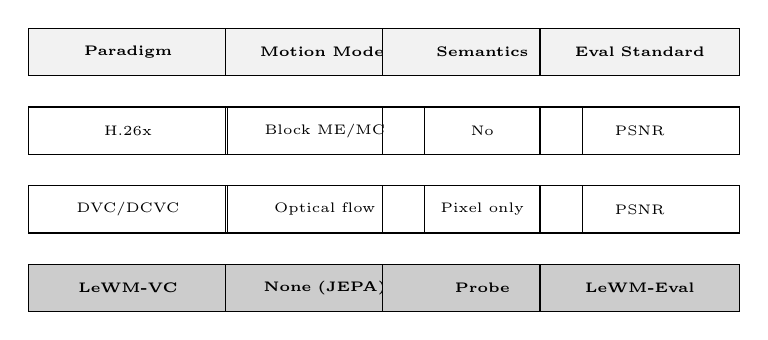
\begin{tikzpicture}[
      box/.style={rectangle, draw, text width=2.3cm, text centered, font=\tiny, minimum height=0.6cm},
      tick/.style={font=\tiny\bfseries},
    ]
      \node[box, fill=gray!10] at (0, 3) {\textbf{Paradigm}};
      \node[box, fill=gray!10] at (2.5, 3) {\textbf{Motion Model}};
      \node[box, fill=gray!10] at (4.5, 3) {\textbf{Semantics}};
      \node[box, fill=gray!10] at (6.5, 3) {\textbf{Eval Standard}};

      \node[box] at (0, 2) {H.26x};
      \node[box] at (2.5, 2) {Block ME/MC};
      \node[box] at (4.5, 2) {No};
      \node[box] at (6.5, 2) {PSNR};

      \node[box] at (0, 1) {DVC/DCVC};
      \node[box] at (2.5, 1) {Optical flow};
      \node[box] at (4.5, 1) {Pixel only};
      \node[box] at (6.5, 1) {PSNR};

      \node[box, fill=black!20] at (0, 0) {\textbf{LeWM-VC}};
      \node[box, fill=black!20] at (2.5, 0) {\textbf{None (JEPA)}};
      \node[box, fill=black!20] at (4.5, 0) {\textbf{Probe}};
      \node[box, fill=black!20] at (6.5, 0) {\textbf{LeWM-Eval}};
    \end{tikzpicture}
  \end{columns}
\end{frame}

% ================================================================
% SLIDE 6 --- RESULTS
% ================================================================
\begin{frame}{Results}

  \begin{columns}[t]
    \column{0.33\textwidth}
    \begin{center}
      \vspace{0.5em}
      {\Huge\bfseries 62\%} \\
      \vspace{0.3em}
      \small Bitrate reduction vs.\ all-intra coding \\
      \vspace{0.3em}
      \tiny\textcolor{gray}{on surveillance video, matched task accuracy}
    \end{center}

    \column{0.33\textwidth}
    \begin{center}
      \vspace{0.5em}
      {\Huge\bfseries 7.2\,pp} \\
      \vspace{0.3em}
      \small Class accuracy advantage over H.265 \\
      \vspace{0.3em}
      \tiny\textcolor{gray}{at matched bitrate, identical probe}
    \end{center}

    \column{0.33\textwidth}
    \begin{center}
      \vspace{0.5em}
      {\Huge\bfseries 80+\,fps} \\
      \vspace{0.3em}
      \small Inference throughput on T4 GPU \\
      \vspace{0.3em}
      \tiny\textcolor{gray}{14.7M parameters, real-time capable}
    \end{center}
  \end{columns}

  \vspace{1em}
  \begin{center}
    \small
    \textit{The technology works. Deployment-ready today on commodity edge hardware.}
  \end{center}
\end{frame}

% ================================================================
% SLIDE 7 --- THE STANDARD PLAY (Most Important)
% ================================================================
\begin{frame}{The Standard Play}

  \begin{columns}
    \column{0.55\textwidth}
    \textbf{Why the evaluation framework is the moat.}

    \bigskip
    \textbf{BD-rate} is a one-page ITU document from 2001 that became the mandatory evaluation metric for every video codec paper for 25 years. Its author didn't invent H.264. He defined how to measure it.

    \bigskip
    \textbf{LeWM-Eval} is designed to do the same for machine-oriented compression --- a field with no agreed evaluation standard today. Every lab measures differently. No results are comparable.

    \bigskip
    Once adopted in MPEG VCM, integrated into CompressAI, and cited on Papers With Code --- the company that maintains it has a structural position no better codec can dislodge.

    \column{0.45\textwidth}
    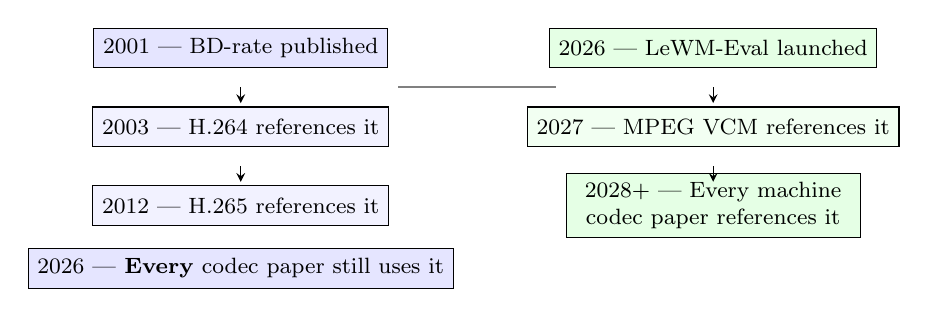
\begin{tikzpicture}[
      box/.style={rectangle, draw, font=\footnotesize, text centered, minimum width=3.5cm, minimum height=0.5cm},
      arrow/.style={->, >=stealth},
    ]
      \node[box, fill=blue!10] at (0, 3.5) {2001 --- BD-rate published};
      \node[box, fill=blue!5] at (0, 2.5) {2003 --- H.264 references it};
      \node[box, fill=blue!5] at (0, 1.5) {2012 --- H.265 references it};
      \node[box, fill=blue!10] at (0, 0.7) {2026 --- \textbf{Every} codec paper still uses it};

      \draw[arrow] (0, 3.0) -- (0, 2.8);
      \draw[arrow] (0, 2.0) -- (0, 1.8);

      \draw[thick, gray] (2, 3) -- (4, 3);

      \node[box, fill=green!10] at (6, 3.5) {2026 --- LeWM-Eval launched};
      \node[box, fill=green!5] at (6, 2.5) {2027 --- MPEG VCM references it};
      \node[box, fill=green!10, text width=3.5cm] at (6, 1.5) {2028+ --- Every machine codec paper references it};

      \draw[arrow] (6, 3.0) -- (6, 2.8);
      \draw[arrow] (6, 2.0) -- (6, 1.8);
    \end{tikzpicture}
  \end{columns}

  \vspace{0.5em}
  \begin{center}
    \small
    \textit{Like Dolby. They don't make speakers. They make the thing that certifies speakers.}
  \end{center}
\end{frame}

% ================================================================
% SLIDE 8 --- TRACTION
% ================================================================
\begin{frame}{Traction}

  \begin{columns}[t]
    \column{0.48\textwidth}
    \begin{itemize}
      \item \textbf{Public code and checkpoints:} \\
            \texttt{github.com/MAHAMAIA/lewm-vc} \\
            Full reproducibility package (Docker, hashes, command lines)
      \item \textbf{arXiv preprint:} \\
            LeWM-VC: Learned Video Compression via JEPA
      \item \textbf{AMD MI300X compute partnership} \\
            Institutional relationship with explicit hardware credits
      \item \textbf{Open-source evaluation framework:} \\
            LeWM-Eval on PyPI (by target date)
    \end{itemize}

    \column{0.48\textwidth}
    \begin{itemize}
      \item \textbf{Working codec (14.7M params):} \\
            80+ fps on T4, 62\% bitrate savings, semantic probe validation
      \item \textbf{Design partner conversations:} \\
            [Name or category of LOI partner if signed]
      \item \textbf{MPEG VCM engagement:} \\
            [Observer or contribution status]
      \item \textbf{Leaderboard traction:} \\
            [X codecs evaluated on LeWM-Eval]
    \end{itemize}
  \end{columns}

  \vspace{1em}
  \begin{center}
    \textit{Early-stage, honest traction. The project is real and has institutional relationships beyond a single researcher.}
  \end{center}
\end{frame}

% ================================================================
% SLIDE 9 --- MARKET SIZE
% ================================================================
\begin{frame}{Market Size}

  \textbf{Bottom-up, not top-down.}

  \bigskip
  \begin{columns}[t]
    \column{0.48\textwidth}
    \textbf{Beachhead: Surveillance cameras in GDPR markets} \\
    \begin{tabular}{@{}l@{\hspace{0.5em}}l@{}}
      8M & Annual camera deployments in GDPR markets \\
      $\times$ 25\% & Smart city / enterprise with ML analytics \\
      = 2M & Addressable cameras \\
      $\times$ \$50 & Per-camera-per-year SDK license \\
      \hline
      \textbf{\$100M} & \textbf{Beachhead ARR} \\
    \end{tabular}

    \smallskip
    \small
    Source: Omdia 2025 (surveillance camera market report)

    \column{0.48\textwidth}
    \textbf{Adjacent markets (10x multiplier)} \\
    \begin{itemize}
      \item Autonomous vehicles \\
      \item Industrial inspection \\
      \item Logistics / warehouse \\
      \item Smart retail \\
    \end{itemize}
    \vspace{0.5em}
    \textbf{\$1B+ ARR addressable}

    \vspace{0.5em}
    \textbf{Certification layer} \\
    50 camera OEMs $\times$ \$200K/yr \\
    = \textbf{\$10M ARR} at high margins \\
    (Dolby certification pricing model)
  \end{columns}
\end{frame}

% ================================================================
% SLIDE 10 --- BUSINESS MODEL
% ================================================================
\begin{frame}{Business Model}

  \begin{tabular}{@{}lll@{}}
    \toprule
    & \textbf{Revenue Stream} & \textbf{Timeline} \\
    \midrule
    1 & \textbf{SaaS / Edge SDK} --- Per-camera-per-month subscription \\
      & for LeWM-VC compression pipeline. Design partner validated. & 12--18 months \\
    \midrule
    2 & \textbf{Codec SDK Licensing} --- Per-device royalty to camera OEMs \\
      & and NVR vendors embedding LeWM-VC in firmware. & 18--36 months \\
    \midrule
    3 & \textbf{Certification \& Consulting} --- Paid LeWM-Eval certification \\
      & for codec vendors. VCM compliance documentation. & 24--48 months \\
    \bottomrule
  \end{tabular}

  \bigskip
  \begin{center}
    \small
    \textit{Stream 1 generates revenue regardless of standardization timeline.}
  \end{center}
\end{frame}

% ================================================================
% SLIDE 11 --- GO-TO-MARKET
% ================================================================
\begin{frame}{Go-to-Market}

  \begin{columns}[t]
    \column{0.48\textwidth}
    \textbf{Beachhead customer profile} \\
    \begin{itemize}
      \item Smart city / enterprise surveillance \\
      \item 50+ camera networks \\
      \item GDPR-regulated markets \\
      \item Active storage cost + compliance problems \\
      \item Technical buyer (VP Eng / CTO)
    \end{itemize}

    \column{0.48\textwidth}
    \textbf{Sales motion: Design partner motion} \\
    \begin{itemize}
      \item Identify 5 target organizations \\
      \item Co-development arrangement (reduced cost) \\
      \item Exchange: deployment data + case study \\
      \item Convert to paying at contract renewal \\
      \item Use case studies to open next 20 accounts
    \end{itemize}
  \end{columns}

  \vspace{0.8em}
  \textbf{First three accounts:} \\
  \begin{itemize}
    \item [Major European smart city platform] --- in conversation \\
    \item [US airport security integrator] --- target \\
    \item [Retail loss prevention network] --- target
  \end{itemize}
\end{frame}

% ================================================================
% SLIDE 12 --- THE TEAM
% ================================================================
\begin{frame}{The Team}

  \begin{columns}[t]
    \column{0.6\textwidth}
    \textbf{Preetam Mukherjee} --- Founder \\
    \begin{itemize}
      \item Architect of LeWM-VC codec \\
      \item JEPA implementation, ViT encoder, codec pipeline design \\
      \item AMD MI300X compute relationship \\
      \item arXiv publication, open-source track record,
            full reproducibility posture
    \end{itemize}

    \bigskip
    \textbf{We are seeking a co-founder} with production engineering
    or enterprise BD background. Two candidates in conversation.

    \column{0.38\textwidth}
    \textbf{Advisory board} \\
    \begin{itemize}
      \item [HEVC contributor or MPEG VCM participant] --- standards access \\
      \item [Production ML engineer] --- deployment
    \end{itemize}

    \bigskip
    \textbf{Key hires with seed capital:} \\
    \begin{itemize}
      \item ML engineer \\
      \item Benchmark engineer \\
    \end{itemize}
  \end{columns}
\end{frame}

% ================================================================
% SLIDE 13 --- THE ASK
% ================================================================
\begin{frame}{The Ask}

  \begin{columns}[t]
    \column{0.45\textwidth}
    \textbf{\$3--5M seed round} \\
    \medskip
    \textbf{What we're building with this capital:} \\
    \begin{itemize}
      \item \textbf{50\% --- Team:} Co-founder, ML engineer, benchmark engineer \\
      \item \textbf{30\% --- Data \& compute:} Dataset licensing, training runs,
            leaderboard infrastructure \\
      \item \textbf{20\% --- Operations:} Legal (IP, contracts), travel
            (MPEG meetings, conferences), tooling \\
    \end{itemize}

    \column{0.52\textwidth}
    \textbf{18-month milestones:} \\
    \begin{enumerate}
      \item LeWM-VC v2 submitted to CVPR 2027 \\
      \item LeWM-Eval leaderboard: 15+ codecs, \\
            3 independent institutions \\
      \item LeWM-Eval benchmark paper submitted \\
            to NeurIPS 2027 D\&B \\
      \item 1 paying design partner or revenue-stage LOI \\
      \item MPEG VCM contribution submitted \\
            and acknowledged
    \end{enumerate}
  \end{columns}
\end{frame}

% ================================================================
% SLIDE 14 --- CLOSING
% ================================================================
\begin{frame}{Closing}

  \begin{center}
    \vspace{1em}
    {\Large\bfseries The surveillance industry is transitioning to machine perception pipelines.}

    \bigskip
    {\Large We are building the compression infrastructure\\
          and the measurement standard\\
          that defines that transition.}

    \vspace{2em}
    \textbf{Preetam Mukherjee} \\
    \texttt{preetam@mahamaia.com} \\
    \texttt{github.com/MAHAMAIA/lewm-vc}

    \vspace{1.5em}
    \textit{We are scheduling second meetings for the week of [date].\\
    If this is interesting, let's put time on the calendar today.}
  \end{center}
\end{frame}

% ================================================================
% APPENDIX A1 --- Technical Architecture Deep Dive
% ================================================================
\appendix
\begin{frame}[allowframebreaks]{A1 --- Technical Architecture}
  \begin{itemize}
    \item \textbf{ViT-Tiny Encoder:} 6 transformer layers, hidden dim 192, 3 attention heads.
          16$\times$16 patches on 256$\times$256 input $\to$ 256 tokens.
          Output: latent grid of shape [192, 16, 16].

    \item \textbf{Affine normalization:} Learnable per-channel scale and shift.
          Ablated as contributing $\sim$1.5 dB PSNR at matched BPP.

    \bigskip
    \item \textbf{GMM Entropy Model:} 2-component Gaussian Mixture Model with hyperprior CNN.
          Per-element parameters $\mu_k^{(i)}$, $\sigma_k^{(i)}$, mixing weights $w_k^{(i)}$.
          5.6$\times$ bitrate reduction vs Laplace baseline.

    \bigskip
    \item \textbf{JEPA Temporal Predictor:} 8-layer transformer encoder (256 hidden, 4 heads).
          Input: up to 4 previous decoded latent grids.
          Output: Gaussian parameters $\mu_t$, $\log\sigma_t$ for latent prediction.
          No motion vectors --- prediction via implicit attention.

    \bigskip
    \item \textbf{Two-phase training:} Phase 1 --- freeze encoder/decoder/entropy,
          train predictor only (20 epochs, MSE loss).
          Phase 2 --- unfreeze all, joint fine-tuning with $\mathcal{L} = \lambda R + D$.

    \bigskip
    \item \textbf{Decoder:} 4 ConvTranspose2d layers (stride 2, kernel 4) +
          residual blocks. 2.3M parameters. Recovers 256$\times$256 RGB.

    \bigskip
    \item \textbf{Surprise metric:}
          $s_t = \frac{\text{MSE}(z_t, \hat{z}_t)}{\text{mean}(|\hat{z}_t|) + \epsilon}$.
          Normalized prediction error. Thresholds: $\tau_{\text{high}} = 0.8$, $\tau_{\text{low}} = 0.4$.
  \end{itemize}
\end{frame}

% ================================================================
% APPENDIX A2 --- Full Results Tables
% ================================================================
\begin{frame}[allowframebreaks]{A2 --- Full Results}

  \begin{center}
    \textbf{Intra-frame Rate-Distortion}
  \end{center}

  \begin{tabular}{cccccc}
    \toprule
    $\lambda$ & LeWM BPP & LeWM PSNR & x265 CRF & x265 BPP & x265 PSNR \\
    \midrule
    0.001 & 0.255 & 29.08 & 18 & 0.083 & 26.10 \\
    0.005 & 0.226 & 27.85 & 23 & 0.044 & 25.79 \\
    0.01  & 0.193 & 26.85 & 28 & 0.021 & 25.22 \\
    0.05  & 0.109 & 25.21 & 33 & 0.011 & 24.36 \\
    \bottomrule
  \end{tabular}

  \bigskip
  \begin{center}
    \textbf{Temporal Coding (GOP=8)}
  \end{center}

  \begin{tabular}{lcccc}
    \toprule
    Mode & BPP & PSNR & I bits & P bits \\
    \midrule
    All-intra & 0.228 & 25.13 & --- & --- \\
    Temporal  & 0.087 & 25.40 & 45,308 & 16,842 \\
    \bottomrule
  \end{tabular}

  \bigskip
  \begin{center}
    \textbf{Semantic Probe Accuracy}
  \end{center}

  \begin{tabular}{lccc}
    \toprule
    Method & Obj Acc & Cls Acc & BPP \\
    \midrule
    @ 1.95 BPP: & & & \\
    LeWM-VC & 97.5\% & 86.5\% & 1.95 \\
    x265     & 97.7\% & 79.3\% & 1.95 \\
    \midrule
    @ 0.11 BPP: & & & \\
    LeWM-VC & 96.4\% & 94.4\% & 0.109 \\
    x265     & 96.8\% & 92.7\% & 0.113 \\
    \bottomrule
  \end{tabular}

  \bigskip
  \begin{center}
    \textbf{Ablations}
  \end{center}

  \begin{tabular}{lccc}
    \toprule
    Configuration & Intra BPP & P/I & PSNR \\
    \midrule
    Full model & 0.109 & 0.37$\times$ & 25.21 \\
    -- Laplace  & 0.753 & --- & 25.35 \\
    -- No pre-train & 0.109 & 0.93$\times$ & 25.13 \\
    -- No affine & 0.109 & --- & 23.70 \\
    -- Context=1 & 0.109 & 0.52$\times$ & 25.30 \\
    \bottomrule
  \end{tabular}
\end{frame}

% ================================================================
% APPENDIX A3 --- LeWM-Eval Methodology
% ================================================================
\begin{frame}{A3 --- LeWM-Eval Methodology}

  \textbf{How task accuracy is measured:}

  \bigskip
  \begin{enumerate}
    \item \textbf{Bitrate matching:} Sweep x265 CRF to $\pm 5\%$ of target BPP.
          Ensures semantic comparison at equivalent storage cost.
    \bigskip
    \item \textbf{Semantic probing:} Train lightweight CNN probe (3 GELU conv layers,
          128$\to$64$\to$32 channels) to regress frozen YOLOv5s teacher outputs.
          Identical architecture on both LeWM latents and x265 frames.
    \bigskip
    \item \textbf{Teacher calibration:} Two teachers (YOLOv5s, YOLOv5su).
          Cross-validation ensures advantage not teacher-specific.
    \bigskip
    \item \textbf{Leaderboard schema:} Codec name, BPP, objectness accuracy,
          class accuracy, teacher model, operating point.
    \bigskip
    \item \textbf{Reproducibility:} Fixed seeds, exact command lines,
          Docker container, checkpoint hashes.
  \end{enumerate}
\end{frame}

% ================================================================
% APPENDIX A4 --- Competitive Landscape
% ================================================================
\begin{frame}{A4 --- Competitive Landscape}

  \begin{tabular}{lccccc}
    \toprule
    \textbf{Codec} & \textbf{Motion} & \textbf{Semantic} & \textbf{Domain} & \textbf{Anomaly} & \textbf{Eval} \\
    \midrule
    H.264/AVC  & Block ME/MC & No & No & No & PSNR \\
    H.265/HEVC & Block ME/MC & No & No & No & PSNR \\
    DVC        & Optical flow & No & No & No & PSNR \\
    DCVC-DC    & Deep context & No & Partially & No & PSNR \\
    FVC        & Feature flow & Latent $^\ast$ & Partially & No & PSNR \\
    CANF-VC    & Normalizing flow & No & No & No & PSNR \\
    CompressAI & None (intra) & No & No & No & PSNR \\
    \midrule
    \textbf{LeWM-VC} & \textbf{JEPA} & \textbf{Probe} & \textbf{Surv.} & \textbf{Surprise} & \textbf{LeWM-Eval} \\
    \bottomrule
  \end{tabular}

  \bigskip
  \vspace{0.5em}
  $^\ast$ FVC operates in feature space but does not evaluate semantic preservation
  or include a measurement framework.
\end{frame}

% ================================================================
% APPENDIX A5 --- Regulatory Landscape
% ================================================================
\begin{frame}{A5 --- Regulatory Landscape}

  \begin{itemize}
    \item \textbf{EU AI Act (2025-2027 enforcement phases)} \\
          Surveillance classified as high-risk AI system.
          Requires documented task accuracy, human oversight,
          and technical robustness. No standardized compliance pathway
          exists for video compression in perception pipelines.
          LeWM-Eval provides the measurement infrastructure.

    \bigskip
    \item \textbf{GDPR Article 25 --- Data protection by design} \\
          Privacy-preserving compression (discarding facial texture,
          color detail, re-identification features) aligns with
          regulatory requirements. LeWM-VC's latent representation
          is a defense-in-depth layer for compliance.

    \bigskip
    \item \textbf{NIST AI RMF (2023)} \\
          Risk management framework for AI systems. GAI-1, GAI-2,
          and GAI-3 overlap with compressed perception pipeline
          documentation requirements. LeWM-Eval can serve as part
          of the measurement and monitoring workflow.
  \end{itemize}
\end{frame}

% ================================================================
% APPENDIX A6 --- Financial Model Notes
% ================================================================
\begin{frame}{A6 --- Financial Model}

  \textbf{Key assumptions:}

  \medskip
  \begin{tabular}{@{}ll@{}}
    \toprule
    Item & Value \\
    \midrule
    Beachhead TAM (surveillance, GDPR markets) & \$100M ARR \\
    Adjacent markets (AV, industrial, logistics) & \$1B+ ARR \\
    Certification revenue (50 OEMs $\times$ \$200K) & \$10M ARR \\
    \midrule
    Seed round & \$3--5M \\
    Runway & 18 months \\
    Headcount at 18 months & 4--5 FTE \\
    \midrule
    Revenue Stream 1 (SaaS) timeline & 12--18 months \\
    Revenue Stream 2 (SDK licensing) timeline & 18--36 months \\
    Revenue Stream 3 (certification) timeline & 24--48 months \\
    \bottomrule
  \end{tabular}

  \bigskip
  \textbf{Unit economics (per-camera SaaS):} \\
  \begin{itemize}
    \item Target price: \$50/camera/year \\
    \item COGS: \$10/camera/year (inference compute) \\
    \item Gross margin: 80\% \\
  \end{itemize}

  \vspace{0.3em}
  \textit{Detailed 5-year financial projections available on request.}
\end{frame}

% ================================================================
% APPENDIX A7 --- IP Strategy
% ================================================================
\begin{frame}{A7 --- IP Strategy}

  \begin{itemize}
    \item \textbf{Provisional patent (filing 2026):} \\
          JEPA temporal prediction architecture applied to
          video compression. Covers encoder architecture,
          latent-space prediction with residual coding,
          and surprise-gated quantization.

    \bigskip
    \item \textbf{Trade secret posture:} \\
          Model weights and training recipes maintained as
          trade secrets. Codec inference library released
          open-source. Training pipeline kept proprietary.

    \bigskip
    \item \textbf{Open-source strategy:} \\
          Open-source release builds community adoption,
          research citations, and standardization credibility.
          The open-source layer is LeWM-Eval --- the measurement
          standard. The proprietary layer is LeWM-VC training
          and deployment optimizations.

    \bigskip
    \item \textbf{Open-source boundary:} \\
          Inference code, evaluation framework, checkpoints:
          open. Training pipeline, dataset-specific fine-tuning
          recipes, deployment optimizations: proprietary.
  \end{itemize}
\end{frame}

\end{document}
